\documentclass[14pt,Diplom]{diplomwork}

\usepackage{fancyvrb}
\renewcommand{\theFancyVerbLine}{\footnotesize\arabic{FancyVerbLine}}
\usepackage[dvips]{color}
\usepackage{tikz}
\usepackage{graphicx}
\usepackage{listings}
\graphicspath{{./img/}}


\newcommand{\alert}[1]{{\color{red}#1}}

\sloppy

\date{2022}
\author{студент МКб-4301-51-00}{Мельков Алексей Константинович}
\advisor{канд. физ.-матем. наук, доцент}{Марков Роман Владимирович}
\title{Разработка модуля интеграции онлайн-сервиса построения графиков и геометрических чертежей в визуальный онлайн HTML-редактор}


\napravlenie{02.03.01}{Математика и компьютерные науки}
\profile{Математические основы компьютерных наук}
\kafedra{фундаментальной математики}{Е.\,М.~Вечтомов}
\department{компьютерных и физико-математических наук}{Н.\,А.~Бояринцева}
\institute{математики и информационных систем}

% ЗАПОЛНЕНИЕ РЕФЕРАТА ПО НОВОМУ ОБРАЗЦУ
%TODO Обязательно впишите ключевые слова
\keywords{HTML, JavaScript, TinyMCE, GeoGebra, Moodle, PHP, API, модуль интеграции}

\annotation{
	\begin{description}
		\item[Объект разработки:] модуль интеграции онлайн-сервиса построения графиков и геометрических чертежей в визуальный онлайн HTML-редактор
		%TODO

		\item[Цель:] определение способностей и готовности самостоятельно решать на современном уровне задачи своей профессиональной деятельности, профессионально излагать специальную информацию, научно аргументировать и защищать свою точку зрения.
		%TODO

		\item[Методы проведения работы:] <Описываются применяемые методы: анализ научной литературы, сравнительный анализ, математическое моделирование, методы математического анализа и т.\,д.>
		%TODO

		\item[Рассматриваются вопросы:] связи онлайн-сервиса построения графиков и геометрических чертежей GeoGebra и визуальный онлайн HTML-редактор TinyMCE
		%TODO
	\end{description}





}
\regtotcounter{figure}
\regtotcounter{table}
\begin{document}

	
\maketitle
\makereferat		% печатаем реферат
\newpage

\tableofcontents


\Chapter{Введение}
Выпускная квалификационная работа посвящена разработке модуля интеграции онлайн-сервиса построения графиков и геометрических чертежей в визуальный онлайн HTML-редактор


\textbf{Актуальность} работы обусловлена оптимизацией времени и удобности написания статей, вопросов, заданий. Данный модуль позволит интегрировать распространенный онлайн-сервис построения графиков и геометрических чертежей GeoGebra в онлайн HTML-редактор TinyMCE, который присутствует на платформе Moodle. Что добавит возможность составления новых тестов, лекций, практических заданий для обучения студентов.

\textbf{Объектом исследования} является изучение API сервисов TinyMCE, GeoGebra, платформы Moodle.

\textbf{Цель работы:} написание плагина для платформы Moodle, который расширит возможности TinyMCE добавлением новой кнопки, которая сможет открыть сервис построения графиков GeoGebra.

Для достижения поставленной цели сформулированы следующие \mbox{\textbf{задачи:}}

\begin{enumerate}
	\item Изучение основ программирования на языке JavaScript
	\item Изучение API GeoGebra, TinyMCE, Moodle
	\item Создание плагина
\end{enumerate}



\textbf{Теоретическая значимость работы} состоит в изучении связи TinyMCE, GeoGebra, Moodle.

\textbf{Практическая значимость работы} состоит в возможности составления новых материалов с использованием GeoGebra.

В целом работа носит \textbf{практический} характер.



\textbf{Структура работы.} Выпускная квалификационная работа, общим объемом \pageref{LastPage}~стр., состоит из введения, двух глав, заключения, библиографического списка.

Первая глава посвящена теоритической части

Вторая глава посвящена практической части


В заключении представлены основные результаты дипломной работы.

В библиографический список включено 10 источников.



\chapter{Теоретическая часть}

\section{Анализ готовых решений}

Существует несколько способов вставки графиков в текстовый редактор в Moodle. Первый способ представлен самой GeoGebra. Они предлагают с сайта построить необходимые графики, затем нажать комбинацию клавиш, что позволит скопировать HTML код. После этого в редакторе TinyMCE есть кнопка редактирования HTML кода, при ее нажатии откроется окно, куда надо вставить скопированные данные.\\
Второй способ – установить плагин Geograph. Он позволяет редактировать апплеты геогебры непосредственно на сайте и сохраняет результат в виде строки base64. Base64 – код, который можно вставить в приложение геогебры, а он раскодируется в нужные параметры. Но существенный минус такого способа заключаются в том, что этот код не вставить в текст, чтобы он преобразовался в график. Еще один минус, что плагин требует установленный на компьютере Java.

\section{Описание своего решения}

В Moodle представлены три онлайн-редактора. Atto, TinyMCE, простой текст. Простой текст - текстовое пространтсво без кнопок, его нельзя изменять. У TinyMCE больше возможностей, при работе с текстом чем у Atto, к примеру, выбор шрифта и размер текста. Поэтому для написания плагина выбран TinyMCE. Среди онлайн сервисов построения графиков и геометрических чертежей была выбрана GeoGebra, так как она популярна и проста для использования. В итоге, предлагается расширить возможности редактора TinyMCE с помощью разработки собственной кнопки, которая при нажатии открывает окно GeoGebra. В этом окне можно построить графики, после чего нажать на внутреннюю кнопку вставки. В результате, все данные перенесутся в текстовую область. Полученный график будет виден при просмотре страницы:

\begin{figure}
	\begin{center}
	\includegraphics[width=0.5\linewidth]{5.png}\caption{нажатие на кнопку}

	\includegraphics[width=0.5\linewidth]{6.png}\caption{построение графика}

	\includegraphics[width=0.5\linewidth]{7.png}\caption{кнопка вставки}

	\includegraphics[width=0.5\linewidth]{8.png}\caption{результат}
	\end{center}
\end{figure}


\section{Необходимые знания}
	Далее будут рассмотрены основы JavaScript, API Moodle, GeoGebra, TinyMCE.
\subsection{основы JavaScript}

\paragraph{JavaScript -}

это язык программирования. Поддерживает объектно-ориентированныйи стили. То есть, программа состоит из компонентов, соответствующих объектам реального мира. Любой реальный объект имеет какие-то свойства (которые могут изменяться или нет с течением времени) и поведение (которое может меняться или нет в зависимости от других условий). 

JavaScript обычно используется как встраиваемый язык для программного доступа к объектам приложений. Наиболее широкое применение находит в браузерах как язык сценариев для придания интерактивности веб-страницам.

\paragraph{Переменные.}
Представляет собой именованную область памяти, к которой можно обращаться через идентификатор для считывания значения
и записи значения. Также у переменной есть тип: 
 \begin{itemize}
	\item Number: любое число, включая десятичные дроби
	\item String: любая группа символов, заключенная в одинарные кавычки: '...' или двойные кавычки "..."
	\item Boolean: этот тип данных имеет только два возможных значения: либо true, либо false. Полезно думать о логических значениях как о переключателях включения и выключения или как об ответах на вопрос “да” или “нет”
	\item Null: этот тип данных представляет намеренное отсутствие значения и представлен ключевым словом null
	\item Undefined: этот тип данных обозначается ключевым словом undefined. Он также представляет отсутствие значения, хотя его использование отличается от null. Отличие в том, что Undefined означает, что данное значение не существует.
	\item Object: коллекция связанных данных
\end{itemize}

\paragraph{Свойства объектов.}
 Когда вводится новый фрагмент данных в программу JavaScript, браузер сохраняет его как экземпляр типа данных. Все типы данных имеют доступ к определенным свойствам, которые передаются каждому экземпляру. Например, каждый экземпляр string имеет свойство length, в котором хранится количество символов в этой строке. Можно получить информацию о свойстве, добавив строку с точкой и именем свойства, к примеру: 
 \begin{verbatim} Console.log('Привет'.length);  выведет в консоль 6 \end{verbatim} 

\paragraph{Методы объектов -}
это действия, которые можно выполнить. Типы данных имеют доступ к определенным методам, которые позволяют обрабатывать экземпляры этого типа данных. Чтобы вызвать метод, необходимо после переменной написать точку, его название, парные скобочки (). К примеру, 
\begin{verbatim} Сonsole.log('привет'.toUpperCase()); выведет в консоль ПРИВЕТ \end{verbatim} 
\paragraph{Функции.}
 В программировании часто используется код для многократного выполнения определенной задачи. Вместо того, чтобы переписывать один и тот же код, можно сгруппировать блок кода вместе и связать его с одной задачей, затем повторно использовать этот блок кода всякий раз, когда нужно выполнить задачу снова. Достигается это с помощью создания функций. Функция - это повторно используемый блок кода, который группирует последовательность инструкций для выполнения определенной задачи.
 
 Как объявляется функция:
 \begin{verbatim} 
 	function Идентификатор(параметры){
 	  тело функции;
 	}
 \end{verbatim} 
 %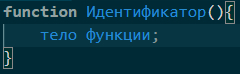
\includegraphics[width=0.5\linewidth]{2.png}\\
 Альтернативным способом можно внести функцию в переменную. Тогда синтаксис объявления поменяется следующим образом:
 \begin{verbatim} 
 	var Переменная = (параметры) => {
 	  тело функции;
 	}
 \end{verbatim} 
 %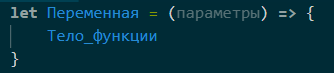
\includegraphics[width=0.5\linewidth]{3.png}\\
  
\paragraph{Объекты.} 
Объекты JavaScript нужны для создания более сложных структур данных. По своей сути, объекты JavaScript представляют собой контейнеры, хранящие связанные данные и функциональные возможности. (набор или
объединение некоторых переменных и функций)\\

Создание объектов, могут быть назначены переменным точно так же, как и любому типу JavaScript. Для обозначения объекта используются фигурные скобки \{\}. Объект можно заполнять неупорядоченными данными. Эти данные организованы в пары ключ-значение. Ключ подобен имени переменной, которое указывает на место в памяти, содержащее значение. Значение ключа может иметь любой тип данных в языке, включая функции или другие объекты.\\

Чтобы создать пару ключ-значение, записываяется имя ключа или идентификатор, за которым следует двоеточие, а затем значение. Каждая пара ключ-значение в объектном литерале разделяется запятой ,:
\begin{verbatim} 
	var Переменная_объекта = {
		ключ: 'что-то',
		'ключ': 123,
	};
\end{verbatim} 
%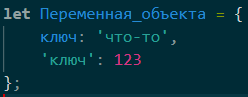
\includegraphics[width=0.5\linewidth]{4.png}\\

Есть два способа получить доступ к свойству объекта. Первый, как и любое свойство - через точку . и название самого свойства. Второй способ получить доступ к значению ключа - использовать обозначение в квадратных скобках, [ ].


\paragraph{}
Для того, чтобы интегрировать JavaScript код в HTML страницу необходимо вставить парный тег <script>. Но также можно подключить JS файл с помощью ссылки на него тем же тегом, c использованием атрибута src, то есть надо указать, где находится этот файл.


\subsection{API MOODLE для плагинов TinyMCE.}
API (Application programming interface) - это инструмент для взаимодействия нескольких программ. API содержит в себе некие «мостики», позволяющие программе А получить доступ к данным из программы Б или к некоторым ее возможностям. Таким образом, программисты могут расширять функциональность своего продукта и связывать его с чужими разработками. Для создания своего плагина TinyMCE необходимо сформировать каталог с его названием. Минимальные файлы для запуска плагина: 
\begin{itemize}
	\item Языковая папка lang с файлом tinyMCE\_ИмяПлагина.php
	\item Папка pix, содержащая значок плагина. Иконка должна называться icon, с расширением .png и размером 20x20 пикселей.
	\item lib.php
	\item version.php
	\item Папка tinymce, в которой хранится иконка кнопки и editor\_plugin.js
\end{itemize}
добавить три php файла, которые обращаются к Moodle.

 \paragraph{version.php}
содержит информацию о версии плагина Moodle
%\textcolor{orange}{<?php} \\
%\textcolor{green}{defined}(\textcolor{red}{'MOODLE\_INTERNAL'}) || (\textcolor{green}{die});\\
%\textcolor{cyan}{\#текущая версия плагина (Дата: ГГГГММДДЧЧ)}\\
%\textcolor{blue}{\$plugin} -> \textcolor{brown}{version} = 2012112900; \\
%\textcolor{cyan}{\#требующиеся версия Moodle (Дата: ГГГГММДДЧЧ)}\\
%\textcolor{blue}{\$plugin} -> \textcolor{brown}{requires} = 2012112900; \\
%\textcolor{cyan}{\#полное имя плагина}\\
%\textcolor{blue}{\$plugin} -> \textcolor{brown}{component} = \textcolor{red}{'tinymce\_ИмяПлагина'}; \\
\begin{Verbatim}
<?php

defined('MOODLE_INTERNAL') || die();

$plugin->version = 2022030209;
 текущая версия плагина (Дата: ГГГГММДДЧЧ)
$plugin->requires = 2012112900; 
 требующиеся версия Moodle (Дата: ГГГГММДДЧЧ)
$plugin->component = 'tinymce_geogebra'; 
 полное имя плагина
\end{Verbatim}

\paragraph{lib.php}
содержит код плагина Moodle, здесь должен находиться по крайней мере класс tinymce\_ИмяПлагина с методом update\_init\_params()\\
%\textcolor{orange}{<?php} \\
%\textcolor{green}{defined}(\textcolor{red}{'MOODLE\_INTERNAL'}) || (\textcolor{green}{die});\\

%\textcolor{green}{class} \textcolor{blue}{tinymce\_ИмяПлагина} \textcolor{green}{extends} editor\_tinymce\_plugin \{ \\
%\textcolor{green}{protected} \textcolor{blue}{\$buttons} = \textcolor{green}{array} (\textcolor{red}{'ИмяПлагина'}); \\

%\textcolor{green}{protected function} \textcolor{blue}{update\_init\_params}(\textcolor{green}{array} \& \textcolor{blue}{\$params}, context %\textcolor{blue}{\$context}, \textcolor{green}{array} \textcolor{blue}{\$options} = \textcolor{green}{null}) \{ \\

%\textcolor{blue}{\$this} -> %\textcolor{yellow}{add\_button\_after}(\textcolor{blue}{\$params},3,\textcolor{red}{'ИмяПлагина'},\textcolor{red}{'spellchecker'});\\

%\textcolor{blue}{\$this} ->\textcolor{yellow}{add\_js\_plugin}(\textcolor{blue}{\$params});\\

%\}\\
%\}\\
\begin{Verbatim}
<?php

defined('MOODLE_INTERNAL') || die();
  
class tinymce_ИмяПлагина extends editor_tinymce_plugin
{
  protected $buttons = array('ИмяПлагина');
  protected function update_init_params(
    array &$params, context $context, array $options = null
  )
  {
    $this->add_button_after(
      $params, $this->count_button_rows($params), 'ИмяПлагина'
    );
    $this->add_js_plugin($params);
  }
}

\end{Verbatim}


\paragraph{tinymce\_ИмяПлагина.php.} 
Файл обязан содержать запись\\
%\textcolor{orange}{<?php} \\
%\textcolor{blue}{\$string}[\textcolor{red}{'pluginname'}] = \textcolor{red}{'ИмяПлагина'};\\
\begin{Verbatim}
<?php
$string['pluginname'] = 'ИмяПлагина'; 
где 'pluginname' нельзя изменять.
\end{Verbatim}

\newpage

\begin{figure}
В результате должен получиться такой каталог:
	\begin{center}
		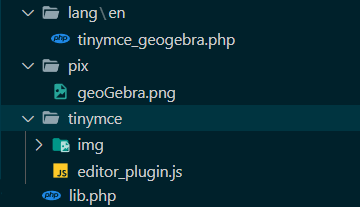
\includegraphics[width=0.5\linewidth]{1.png}\caption{каталог плагина}
	\end{center}
\end{figure}


\subsection{API Tinymce}
Чтобы вставить TinyMCE редактор в HTML страницу надо добавить следующие скрипты:
\begin{Verbatim}
<script 
  src="https://cdn.tiny.cloud/1/no-api-key/tinymce/5/tinymce.min.js" 
  referrerpolicy="origin">
</script>
\end{Verbatim}
Эта строка ссылает страницу на сайт редактора.
\begin{Verbatim}
<script>
  tinymce.init({
  });
</script>
\end{Verbatim}
Этот скрипт запускает TinyMCE. Так как в Moodle уже загружен редактор, и расширяются его возможности, то эти скрипты не нужны. В итоге изменяются параметры init.
\subsection{API Geogebra}
Чтобы на своей странице загрузить GeoGebra, необходимо добавить несколько скриптов и место, куда будет добавляться приложение. Сначала нужно, сделать ссылку на источник GeoGebra: 
\begin{Verbatim}
<script src="https://www.geogebra.org/apps/deployggb.js"></script>
\end{Verbatim}
Затем создадим контейнер, куда вставится приложение:
\begin{Verbatim}
<div id="ggb-element"></div>
\end{Verbatim}
Теперь требуется задать параметры и открыть окно GeoGebra:
\begin{Verbatim}
<script>  
  var params = 
    {
      "appName": "graphing",
      "width": 800,
      "height": 600,
      "showToolBar": true,
      "showAlgebraInput": true, 
      "showMenuBar": true 
    };
  var applet = new GGBApplet(params, true);
  window.addEventListener("load", function() { 
    applet.inject('ggb-element');
  });
</script>
\end{Verbatim}
Разберем параметры:

\begin{itemize}
	\item appName - тип вычислений. Можно выбрать graphing (построение графиков), geometry (геометрия), 3d.
	\item width, height - высота и ширина окна в пикселях.
	\item showToolBar, showAlgebraInput, showMenuBar - отображение инструментов и панелей. Если true - отображаются, если false - скрыты
\end{itemize}

После создается GGBApplet с указанными параметрами. Также при загрузке страницы, срабатывает событие добавления GGBApplet в div контейнер с id 'ggb-element'.


 
\chapter{Практическая часть}
В этой главе будут рассмотрены файлы плагина с кодом и пояснения к ним. 
\section{editor\_plugin.js}
Главный файл модуля интеграции, так как именно в нем описывается добавление нестандартной кнопки, а также здесь задается её функция. Этот файл написан на языке JavaScript. Он из себя представляет большую функцию, в которой содержатся два метода: tinymce.create() и tinymce.PluginManager.add().

\subsection{tinymce.create()}
Этим методом создается объект. Сначала объявляется его идентификатор, затем описывается тело класса.

\begin{verbatim} 
tinymce.create("tinymce.plugins.geogebra", {
  /**
  * @param {tinymce.Editor} ed 
  * @param {string} url 
  */
  ...
}
\end{verbatim}

\begin{itemize}
	\item   @param \{tinymce.Editor\} ed  - тег @param позволяет указать тип, имя и описание параметра функции. В данном случае, параметр ed объявлен типом tinymce.Editor. Это экземпляр переменных редактора, в котором инициализируется плагин.
	\item @param {string} url - параметр, который представлен строкой. Абсолютный URL-адрес, по которому находится плагин.
\end{itemize}

\paragraph{init}
 ключ-функция объекта, которая срабатывает при загрузке веб-страницы.
\begin{verbatim} 
 init: function (ed, url) {
   ed.addCommand("mceGeogebra", function () {
     ed.windowManager.open(
       {
         file: ed.getParam("moodle_plugin_base") + 
           "geogebra/geogebra.php",
         width:
           window.outerWidth - 100 +
           parseInt(ed.getLang("geogebra.delta_width", 0)),
         height:
           window.outerHeight - 250 +
           parseInt(ed.getLang("geogebra.delta_height", 0)),
         inline: 1,
       },
       {
         plugin_url: url,
       }
     );
   });
 
   ed.addButton("geogebra", {
     title: "GeoGebra Plugin",
     cmd: "mceGeogebra",
     image: url + "/img/geoGebra.gif",
   });
 }
\end{verbatim}
 init содержит два входных параметра ed, url. В ней вызывается метод addCommand, который аналогичен init, имеет название команды и обработчик события. Но ed.addCommand это функция, а не объект. Именно здесь задается логика плагина.

\begin{itemize}
	\item ed.windowManager.open(). Открывает диалоговое окно с конфигом, прописанным в параметре функции. Рассмотрим его подробнее. File - абсолютный путь, того что откроет кнопка, при нажатии. В этом случае, открывается php-страница, которая будет рассмотрена ниже. Width, Height - высота, ширина открывающегося окна. Plugin\_url - ссылка на плагин.
	\item ed.addButton(). Добавляет кнопку. Title - текст, который будет отображаться, при наведении на кнопку. Cmd - то, что выполнит кнопка. Image - ссылка на картинку, которая будет отображаться на кнопке.
\end{itemize}

\paragraph{getInfo.}

Второй ключ - функция. При вызове возвращает информацию о плагине.
\begin{verbatim}
getInfo: function () {
  return {
    longname: "GeoGebra plugin",
    author: "Alexei Melkov",
    authorurl: "alekseymelkov@gmail.com",
    infourl: "alekseymelkov@gmail.com",
    version: "1.061",
  };
},
\end{verbatim}

\subsection{tinymce.PluginManager.add()}
 Регистрирует собственный плагин в TinyMCE, используя PluginManager. PluginManager.add() принимает строку для идентификатора плагина и объект, содержащую код для инициализации плагина.
 \begin{verbatim}
 tinymce.PluginManager.add("geogebra", tinymce.plugins.geogebra);
 \end{verbatim}
 Идентификатор "geogebra" и переданный объект tinymce.plugins.geogebra, который был создан выше с помощью метода tinymce.create().
 
\section{geogebra.php}
Страница, которая открывается при нажатии на кнопку. Она написана на языке PHP. Вначале записан PHP код, который при обработке нажатия, вставится в заголовок диалогового окна.

\begin{verbatim}
<?php

define('NO_MOODLE_COOKIES', true);

require('../../../../../config.php');

$PAGE->set_context(context_system::instance());
$PAGE->set_url('/lib/editor/tinymce/plugins/geogebra/geogebra.php');
$PAGE->set_title(get_string('title', 'tinymce_geogebra'));
$PAGE->set_pagelayout('embedded');

$editor = get_texteditor('tinymce');
$plugin = $editor->get_plugin('geogebra');

$PAGE->requires->js(new moodle_url
  ($editor->get_tinymce_base_url() . '/tiny_mce_popup.js'));
$PAGE->requires->js(new moodle_url
  ($plugin->get_tinymce_file_url('js/dialog.js')));

echo $OUTPUT->header();

?>
\end{verbatim}
define - определение константы.\\
require - включает и выполняет указанный файл.\\
\$PAGE - экземпляр moodle\_page, который хранит всю информацию и используется библиотекой вывода \$OUTPUT при отображении страницы.\\
set\_context, set\_url, set\_title, set\_pagelayout - по API Moodle выставляются параметры диалогового окна.\\
После получаем доступ к плагину, чтобы экспортировать нужны файлы.



Потом инициализируется контейнер с GeoGebra и пятью кнопками. Параметры GeoGebra такие же как при описании API. Кнопки делятся на меняющие режим GeoGebra и обновляющие диалоговое окно. Обработчики событий этих кнопок, добавлены в отдельный файл dialog.js, кроме нажатия на кнопку отмены. Она использует стандартный метод close класса tinyMCEPopup.

\begin{verbatim}
  
  <script src="https://www.geogebra.org/apps/deployggb.js"></script>
  <script>
    var params = {
      appName: 'graphig', 
      width: window.outerWidth,
      height: window.outerHeight - 250, 
      showToolBar: true, 
      showAlgebraInput: true, 
      showMenuBar: true,
    };
    var applet = new GGBApplet(params, true);
    window.onload = function () {applet.inject('ggb-element');};
  </script>
  
  <div id="ggb-element">
  </div>
  <p>
    <div>
      <input 
        type="button" id="graphig" name="graphig" 
        value="graphig" onclick="GeoDialog.reloadGraphig();"
      />
      <input
        type="button" id="geometry" name="geometry" 
        value="geometry" onclick="GeoDialog.reloadGeometry();"
      />
      <input type="button" id="3d" name="3d"
       value="3d" onclick="GeoDialog.reload3d();"
      />
      <input type="button" id="editing" name="editing"
       value="Редактировать" onclick="GeoDialog.loadLastGGB();"
      />
      <input type="button" id="insert" name="insert"
       value="Вставить" onclick="GeoDialog.insert();"
      />
      <input type="button" id="cancel" name="cancel"
       value="Отмена" onclick="tinyMCEPopup.close();"
      />
    </div>
  </p>  
\end{verbatim}

Затем добавляется подвал (футер) страницы.
\begin{verbatim}
<?php
echo $OUTPUT->footer();
\end{verbatim}

\section{dialog.js}
В этом файле создаются обработчики событий кнопок. Все они хранятся в объекте GeoDialog.
\begin{verbatim}
var GeoDialog = {
  insert: function () {
    var content = tinyMCE.activeEditor.getContent();
    if (content.indexOf("<div id='applet_container'></div>") == -1) 
    {
      tinyMCEPopup.editor.execCommand(
        "mceInsertContent",
        false,
        "<div id='applet_container'></div>"
      );
    }
  var divGgb = document.getElementsByClassName(
    "appletParameters notranslate"
  )[0];
  var appName = divGgb.getAttribute("data-param-appname");
  var code = ggbApplet.getBase64();
  var width = 1920;
  var inserted =
    "<!-- begin -->" +
    "<script type='text/javascript' 
      src='https://www.geogebra.org/apps/deployggb.js'>
    </script>" +
    "<script type='text/javascript'>var params={ appName:" +
    `'${appName}'` +
    ", width:" +
    `'${width}'` +
    ", showToolBar: false, scaleContainerClass: 'qtext',
    showAlgebraInput: false, showZoomButtons: false, 
    autoHeight: true, showMenuBar: false, ggbBase64:" +
    `'${code}'` +
    "};var applet = new GGBApplet(params, true);" +
    "window.onload = function () {applet.inject('applet_container');};" +
    "</script>" +
    "<!-- end -->";
  var begin = content.indexOf("<!-- begin -->");
  if (begin != -1) {
    var end = content.indexOf("<!-- end -->");
    content =
    content.substring(0, begin)
     + inserted 
     + content.substring(end + 12);
    tinyMCE.activeEditor.setContent(content);
  } 
  else tinyMCEPopup.editor.execCommand(
    "mceInsertContent", false, inserted
  );
  tinyMCEPopup.close();
},
\end{verbatim}
insert - функция, которая вставляет все изменения из приложения GeoGebra в текстовую область редактора с помощью HTML кода. При нажатии на кнопку, сначала вся текстовая область редактора записывается в переменную content. Идет проверка на наличие контейнера с айди "applet\_container". Если его нет в content, то он создается. После с помощью библиотеки jQuery достаются параметры GeoGebra, Base64 код, размер ширины окна. Все эти данные понадобятся при вставке HTML кода. Формируется строковая переменная inserted. В ней записываются скрипты вставки аплета GeoGebra. Для того чтобы заменить нужную часть кода, а не переписывать весь content, он ограничен комментариями <!-- begin --> и <!-- end -->. Если HTML код вставляется не первый раз, а уже существует, тогда по этим меткам он заменится настоящим, иначе внесется первая запись.

\begin{verbatim}
loadLastGGB: function () {
  var content = tinyMCE.activeEditor.getContent();
  var begin = content.indexOf("ggbBase64");
  if (begin != -1) {
    begin = content.indexOf("ggbBase64") + 11;
    var end = content.indexOf("var applet") - 3;
    appName = content.slice(
      content.indexOf("appName") + 9,
      content.indexOf("width") - 3
    );
    var code64 = content.slice(begin, end);
    var params = {
      appName: `'${appName}'`,
      showToolBar: true,
      showAlgebraInput: true,
      showMenuBar: true,
    };
  } else {
    window.alert("В текстовой области нет аплета GeoGebra!");
  }
  var applet = new GGBApplet(params, true);
  window.onload = function () {
    applet.inject("ggb-element");
  };
  ggbApplet.setBase64(code64);
  },
\end{verbatim}
loadLastGGB - функция, которая срабатывает при нажатии на кнопку "редактировать". Ее смысл - обновить окно вставки предыдущими параметрами GeoGebra. Сначала все содержимое текстовой области записывается в переменную content. Затем в коде ищутся ключевые метки ggbBase64 и var applet. Это начало и конец Base64 кода, который преобразовывает строку символов в график. Если метки находятся, тогда из контента достаются тип аплета и Base64, а потом обновляется окно. Если нет меток, то выводится предупреждение на экран, что в текстовой области нет аплета GeoGebra.

\begin{verbatim}
reloadGraphig: function () {
  var params = {
    appName: "graphig",
    showToolBar: true,
    showAlgebraInput: true,
    showMenuBar: true,
  };
  var applet = new GGBApplet(params, true);
  applet.inject("ggb-element");
},
\end{verbatim}

\newpage

\begin{itemize}

	\begin{figure}
		reloadGraphig, reloadGeometry, reload3d - похожие функции, которые вызывают прогрузку приложения GeoGebra в id "ggb-element". Вся их разница в параметре appName. То есть, загрузка разных режимов GeoGebra. Graphig - график, Geometry - геометрия, 3d - 3д режимы. У всех режимов есть ввод функций с помощью калькулятора, но есть различия в инструментариях:\\
			
			\item Graphig, так как это режим для построения графиков, то инструменты помогают расставлять точки, искать корни, находить пересечение, исследовать функции.
			\begin{center}
				\includegraphics[width=1\linewidth]{9.png}\caption{графический режим GeoGebra}
			\end{center}
		\end{figure}
	
	
		\item Geometry - режим для построения геометрических фигур. В нем есть инструменты как для их построения, так и для работы с объектами, к примеру, скрыть или удалить.
		\begin{figure}
			\begin{center}
				\includegraphics[width=1\linewidth]{10.png}\caption{геометрический режим GeoGebra}
			\end{center}
		\end{figure}


		\begin{figure} 
			\item 3d - режим для работы в трехмерном пространстве. Поэтому инструменты направлены на помощь построения объектов в трех измерениях.
			\begin{center}
				\includegraphics[width=1\linewidth]{11.png}\caption{3д режим GeoGebra}
			\end{center}
		\end{figure}
\end{itemize}



	  



\Chapter{Заключение}
При написании выпускной квалификационной работы по теме "Разработка модуля интеграции онлайн-сервиса построения графиков и геометрических чертежей в визуальный онлайн HTML-редактор" были изучены:
\begin{itemize}
	\item основы программирования на языке JavaScript;
	\item API сервиса построения графиков и чертежей GeoGebra;
	\item API онлайн HTML-редактора TinyMCE;
	\item создание собственного плагина на платформе Moodle для TinyMCE;
\end{itemize}
В ходе работы были достигнуты поставленные задачи, разработан модуль интеграции GeoGebra в TinyMCE.\\
Результатом проделанной работы является плагин GeoGebra для платформы Moodle, который можно загрузить по ссылке: https://github.com/markovrv/moodlegeo


\begin{thebibliography}{99}
\bibitem{Book1} Заяц, А. М. Проектирование и разработка WEB-приложений. Введение в frontend и backend разработку на JavaScript и node.js : учебное пособие для спо / А. М. Заяц, Н. П. Васильев. — 2-е изд., стер. — Санкт-Петербург : Лань, 2022. — 120 с. 
\bibitem{Book5} Васильев, А. Н. JavaScript в примерах и задачах / А. Н. Васильев.– Москва :
Издательство «Э», 2017. – 720 с.	
\bibitem{Book2} Документация HTML онлайн-редактора TinyMCE [Электронный ресурс] Режим доступа: URL: https://www.tiny.cloud/docs/api/ , свободный
\bibitem{Book3} Page API Moodle [Электронный ресурс] Режим доступа: URL: https://docs.moodle.org/dev/Page\_API , свободный
\bibitem{Book4} Создание своего плагина TinyMCE для Moodle  [Электронный ресурс] Режим доступа: URL: https://docs.moodle.org/dev/Creating\_a\_Moodle\_specific\_TinyMCE\_plugin , свободный
\bibitem{Book5} API сервиса построения графиков и чертежей GeoGebra [Электронный ресурс] Режим доступа: URL: https://wiki.geogebra.org/en/Reference:GeoGebra\_Apps\_API , свободный
\bibitem{Book5} Руководство с работой фреймворка JavaScript - jQuery [Электронный ресурс] Режим доступа: URL: https://habr.com/ru/post/38208/ , свободный
\bibitem{Book5} Словарь тегов языка HTML и его атрибутов [Электронный ресурс] Режим доступа: URL: http://htmlbook.ru/ , свободный
\bibitem{Book5} Справочник языка PHP [Электронный ресурс] Режим доступа: URL: https://www.php.net/manual/ru/langref.php	 , свободный
\bibitem{Book5} Электронный курс для знакомства с JavaScript [Электронный ресурс] Режим доступа: URL: https://www.codecademy.com/learn/introduction-to-javascript	 , свободный
\end{thebibliography}

 


\end{document}
